\subsection{User Study}\label{sec:user}

\begin{figure*}
     \centering
     \begin{tabular}{ccc}
		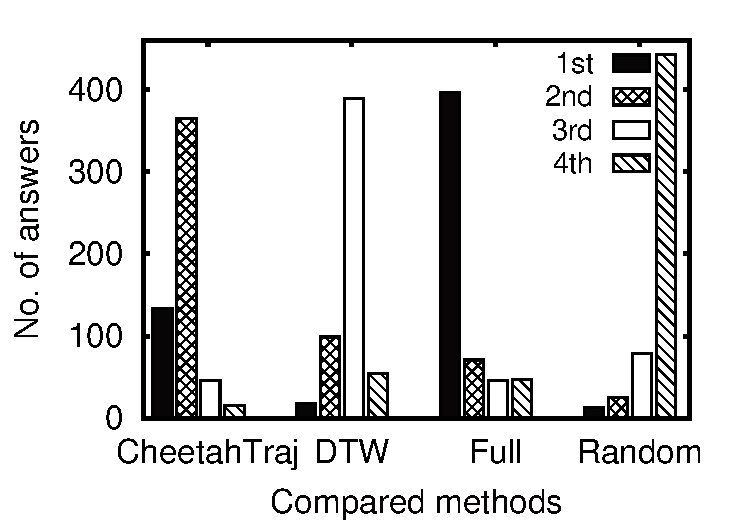
\includegraphics[width=0.6\columnwidth]{pictures/user_study/quality}
		&
		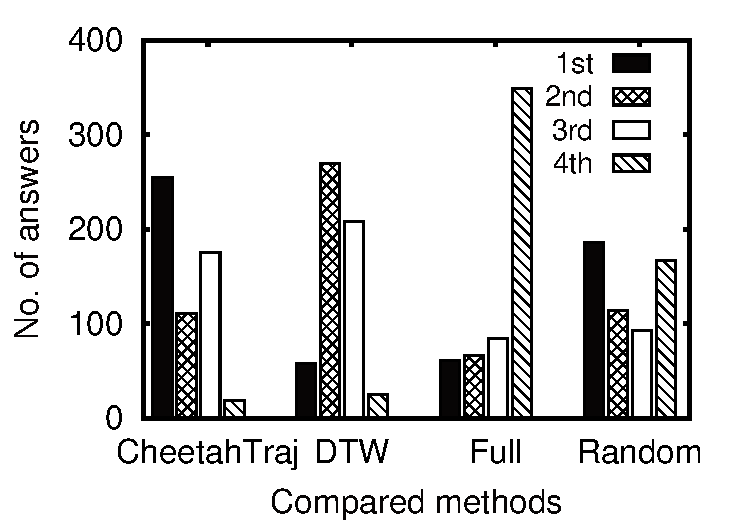
\includegraphics[width=0.6\columnwidth]{pictures/user_study/clutter}
        &
        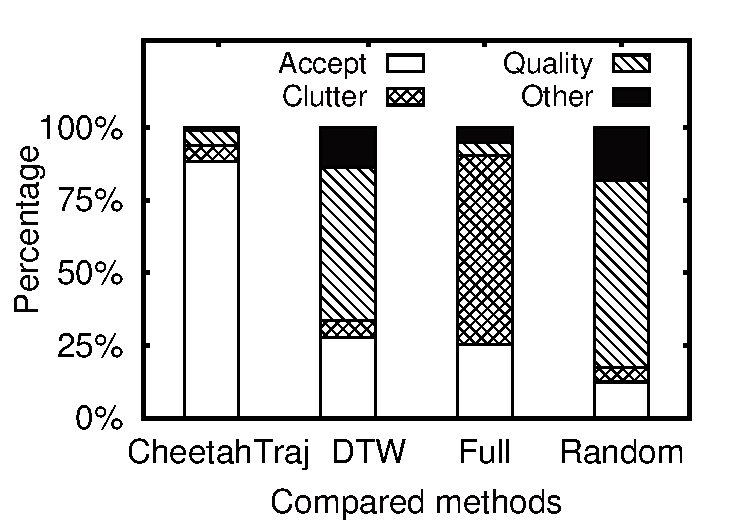
\includegraphics[width=0.6\columnwidth]{pictures/user_study/accept}
		\\
		(A) T1: visual quality study
		&
		(B) T2: visual clutter study
        &
        (C) T3: acceptable visualization study
	\end{tabular}
	\caption{User study results of different visualization methods}
	\label{fig:userstudy}
    \trim
\end{figure*}

In this part, we conduct a user study to evaluate the quality of visualizations generated by different methods objectively.

\stitle{Settings}
We recruited 35 participants with 10 females, 25 males, aged 19 to 31 with a mean of 24.78 for the user study. 
The user study is conducted on the \pt{} and \sz{} datasets, and four visualization methods are investigated, i.e., $\full$, $\rand$, $\mathsf{DTW}$ and $\avats$. We manually select 22 \textit{center points} in the two datasets and define 3 \textit{visualization scales} including:
large-scale region (with zoom level smaller than 13), middle-scale region (with zoom level between 13 and 15), small-scale region (with zoom level larger than 15). For each center point and at each visualization scale, we generate a \textit{comparable visualization group}, which includes one visualization generated by each of the 4 methods. This results in 66 comparable groups (22 center points $\times$ 3 scales) and 264 visualization results (66 comparable groups $\times$ 4 visualizations).

We are interested in the visual quality and visual clutter of the visualizations, and hence designed three tasks for a comparable group:
\begin{itemize}
	\item Task 1 (T1): rank the visualizations in a group from the highest visual quality to the lowest visual quality by 1st, 2nd, 3rd, and 4th.
	\item Task 2 (T2): rank the visualizations in a group from the least visual clutter to the most severe visual clutter by 1st, 2nd, 3rd, and 4th.
	\item Task 3 (T3): select the visualizations considered acceptable (multiple choices allowed) and choose the reason for the visualizations considered unacceptable. We provide three reasons including ``severe visual clutter", ``poor visual quality" and ``others".
\end{itemize}

The user study system is a web-based platform, in which all visualizations are displayed with a resolution of 450*300.


\stitle{User study procedure} When the participants enter the user study system, they are given a tutorial on how to conduct the tasks to get familiar with the interface and tasks.
For each participant, we randomly select 16 comparable groups.
Thus, we obtain $35 \times 16 = 560$ results for each task.
For each comparable group, the 4 visualizations (\textit{without specifying generated by which method}) in it are displayed on the same web-page and a participant is required to perform task T1, T2 and T3 by inspecting them.


\stitle{Result analysis} Figure~\ref{fig:userstudy}(A) reports the visual quality ranking of the 4 methods in T1. 
The results show that $\full$ ranks the 1st in most cases while $\avats$ usually ranks 1st or 2nd, i.e., the percentage of $\avats$ ranks top-2 among 4 methods is $88.9\%$. 
In contrast, $\mathsf{DTW}$ and $\rand$ rank 3rd and 4th at most times. 
This suggests that the visualizations generated by $\avats$ are more appealing to the participants than $\mathsf{DTW}$ and $\rand$. 
We also observed that the participants tend to rank $\avats$ before $\full$ for large-scale regions with  many trajectories, and the other way for smaller regions. 


Figure~\ref{fig:userstudy}(B) reports the anti-visual clutter ranking of the 4 methods in T2. 
The results show that visual clutter is most severe for $\full$, ranking 4th in most cases (349 over 560). With sampling, $\mathsf{DTW}$ usually rank 2nd and 3rd but $\rand$ ranks 4th for a considerable number of times as it tends to create clutter in the dense regions.    
$\avats$ is the most successful in reducing visual clutter, ranking 1st in 255 out of the 560 cases and ranking 4th for only 19 cases.    



We report the frequency each of the 4 methods is selected as acceptable and why a method is not selected in T3 using bar chart in Figure~\ref{fig:userstudy}(C). 
Each column corresponds to a method, and from bottom to top, the lengths of the bars indicate the percentage of participants choosing ``acceptable'', ``not acceptable due to visual clutter'', ``not acceptable due to poor visual quality'' and ``not acceptable for other reasons''. 
The results show that $\avats$ is regarded acceptable for about 88.2\% of the cases, and the other methods have significantly lower acceptance rate than $\avats$. 
Specifically, $\mathsf{DTW}$ and $\rand$ have low acceptance rate mainly due to poor visual quality while $\full$ suffers from severe visual clutter.





